% IEEE Journal of Biomedical and Health Informatics -- manuscript source.
% Compile on Overleaf (IEEEtran is built in) or with a local TeX Live:
%   pdflatex manuscript && pdflatex manuscript
% Items marked \pending{...} must be filled from the study run before submission.
\documentclass[journal]{IEEEtran}
\usepackage{amsmath,amssymb}
\usepackage{booktabs}
\usepackage{array}
\usepackage{graphicx}
\usepackage{tikz}
\usetikzlibrary{arrows.meta,positioning,fit}
\usepackage{xcolor}
\usepackage[hidelinks]{hyperref}
\newcommand{\pending}[1]{\textcolor{red}{[PENDING: #1]}}

\begin{document}

\title{Context-Conditioned Supervision for Clinical Language-Model Assistance: A Dual-Lobe Architecture with Evidence-Gated Release and Identity-Blind Inference}

\author{Anas~Alsawy%
\thanks{A. Alsawy is with \pending{affiliation} (e-mail: anasalsawy@gmail.com).}%
\thanks{This work is a substantially new manuscript; an earlier concept note (JBHI-06009-2026) was declined at editorial screening.}}

\markboth{IEEE Journal of Biomedical and Health Informatics}{Alsawy: Context-Conditioned Supervision for Clinical LLM Assistance}

\maketitle

\begin{abstract}
Language-model assistants answer the question a clinician asks, yet the safety-critical fact is often absent from the question: an analgesic dose is requested for a patient whose record shows advanced kidney disease. Verifiers, judges and guardrails check the answer against the question and inherit its blind spot. We specify, implement and evaluate a dual-lobe architecture in which a primary lobe answers from a de-identified record while a supervisory lobe, required to run on local infrastructure, reads the whole record before and independently of the answer, then audits the answer. Every supervisory finding must cite numbered record facts with verbatim quotes; citations are verified deterministically, and a seven-rule release gate lets only evidence-grounded critical or major findings interrupt the clinician, failing closed when supervision fails. A per-request privacy session replaces identifiers with random tokens held in an encrypted vault without a plaintext index, shifts dates, monitors every outbound payload by destination, and destroys its keys after each request. The gate satisfies seven safety invariants over all 50\,568 enumerated input configurations. On a 133-case benchmark with 626 planted identifiers, deterministic de-identification removed 624 with no defects, leaving two uncued place names for the local supervisory sweep, and delivered all 385 clinical values unchanged. A paired three-arm study (primary only; conventional answer verifier; context-conditioned supervisor) with matched hazard/no-hazard twins and blinded clinician adjudication measures omission detection and false alarms: \pending{headline results}.
\end{abstract}

\begin{IEEEkeywords}
Clinical decision support, large language models, patient safety, AI verification, de-identification, privacy, human--AI interaction.
\end{IEEEkeywords}

\section{Introduction}
\IEEEPARstart{A}{} large language model (LLM) used as a clinical assistant behaves like a gate that opens only to the right words: its knowledge is available when the clinician formulates a precise inquiry, and silent otherwise. We call this the \emph{open-sesame} problem. It shifts to the clinician the burden of anticipating every risk factor before asking. When a clinician asks for an ibuprofen dose for a patient whose record shows an eGFR of 28\,mL/min/1.73\,m$^2$ on an ACE inhibitor and a loop diuretic, a model that answers the dose question correctly has still failed the patient. Such omissions are a recognised mechanism of error: premature closure on an initial frame is among the most common cognitive contributors to diagnostic error \cite{graber2005}.

LLMs encode substantial clinical knowledge \cite{singhal2023,singhal2025,nori2023} but also produce fluent unsupported content \cite{pal2023}. The dominant safety mechanisms check outputs: AI-feedback critique \cite{bai2022}, self-refinement \cite{madaan2023,shinn2023}, self-consistency \cite{wang2023}, chain-of-verification \cite{dhuliawala2024}, trained verifiers \cite{cobbe2021,lightman2024}, LLM judges \cite{zheng2023}, guardrails \cite{inan2023,rebedea2023} and multi-agent debate \cite{du2024,irving2018}. They are conditioned on the answer or on the shared question, and so do not, by design, ask what the question failed to ask. Rule-based clinical decision support (CDS) scans records proactively \cite{bates2003,sutton2020} but is limited to encoded rules and suffers alert fatigue and high override rates \cite{vandersijs2006,ancker2017}. A second barrier is data protection: identifiable records cannot generally be sent to external model providers, and extraction of training data from LLMs is documented \cite{carlini2021}.

As an informal analogy, experienced clinicians rely on a background monitor that notices what the conscious line of reasoning did not ask. We do not claim a neural mechanism; the analogy motivates an explicit engineering separation between a component that answers and a component that watches the whole context. The contributions of this paper are:
\begin{enumerate}
\item \emph{Context-conditioned supervision.} A supervisory lobe reads the entire record before and independently of the answer, to surface omitted hazards while avoiding anchoring on the generator's framing \cite{tversky1974}. A same-model answer-verifier comparison arm isolates this design choice.
\item \emph{A deterministic, verified control layer} comprising citation grounding, verdict rules and a seven-rule release gate that implements an explicit disagreement policy (evidence-gated interruption; neither lobe overrides the other), verified exhaustively.
\item \emph{Identity-blind inference with privacy-asymmetric lobes.} The supervisor must be local, which keeps supervision on-premises and lets it act as residual de-identifier for text about to leave; the answering model sees only a tokenised, date-shifted view, and every request ends with destruction of its keys.
\item \emph{An evaluation apparatus} with a provenance-documented benchmark including matched hazard/no-hazard twins, planted identifiers, paired arms, a leak probe in every run, and blinded clinician adjudication, reported following DECIDE-AI \cite{vasey2022} and TRIPOD-LLM \cite{gallifant2025}.
\end{enumerate}

\section{Related Work}
Table~\ref{tab:related} positions the approach. Self-correction without external feedback is unreliable \cite{huang2024}, motivating a separate supervisor with no shared context. The closest structural analogue is trusted monitoring in AI control \cite{greenblatt2024}, where a trusted, possibly weaker model supervises an untrusted, more capable one; we apply the asymmetry to clinical omission and to data protection. Clinical multi-agent systems \cite{tang2024,kim2024} have role-played specialists deliberate on the same question, sharing its framing. Unlike rule-based CDS, the supervisor can act on hazards carried by free text, but is expected to be less reliable than a curated rule base for well-encoded interactions; rule outputs can therefore be supplied to it as retrieved knowledge \cite{lewis2020,zakka2024}. Automation bias \cite{goddard2012,parasuraman1997} and sycophancy \cite{sharma2024} are treated as design constraints.

\begin{table*}[!t]
\caption{Supervisory approaches compared on dimensions relevant to omission.}
\label{tab:related}
\centering
\footnotesize
\begin{tabular}{@{}p{3.6cm}p{3.1cm}p{2.3cm}p{3.4cm}p{3.3cm}@{}}
\toprule
Approach & Conditioned on & Independent of framing & Evidence required to object & Disagreement handling\\
\midrule
Self-refinement / correction \cite{madaan2023,shinn2023,huang2024} & own answer & no & none & generator revises\\
Chain-of-verification \cite{dhuliawala2024} & own claims & partly & none formal & generator revises\\
Trained verifiers \cite{cobbe2021,lightman2024} & answer (steps) & yes & none (score) & rerank / reject\\
LLM-as-judge \cite{zheng2023} & answer vs rubric & yes & none (score) & score\\
Guardrails \cite{inan2023,rebedea2023} & policy categories & yes & none & block / allow\\
Debate; clinical multi-agent \cite{du2024,irving2018,tang2024,kim2024} & shared question & no / limited & informal & consensus or judge\\
Trusted monitoring \cite{greenblatt2024} & untrusted actions & yes & suspicion score & audit / replace\\
Rule-based CDS \cite{bates2003,vandersijs2006,sutton2020} & order + structured record & yes & encoded rule & interruptive / passive\\
\textbf{This work} & \textbf{whole record, before the answer; then the answer} & \textbf{yes} & \textbf{cited facts, verbatim quotes, retrieved IDs; machine-checked} & \textbf{evidence-gated interruption; clinician arbitrates}\\
\bottomrule
\end{tabular}
\end{table*}

\section{Architecture}
Fig.~\ref{fig:arch} shows the information flow. The record is flattened into numbered facts $F_1,\dots,F_n$ with stable paths; identifier fields are removed and a date of birth becomes an age. The primary lobe $A$ (which may delegate sub-tasks to temporary workers) answers from this view and may run on any provider. The supervisory lobe $B$ runs locally in three roles: $B_0$ sweeps outbound text for residual identifiers; $B_1$ scans the whole record concurrently with $A$ and without seeing $A$'s answer; $B_2$ audits $A$'s exact answer against the record and against $B_1$'s scan. $B$ inherits an anti-deception protocol that classifies claims as observed, inferred, assumed or unknown, requires positive evidence, and fails closed. $B$ never rewrites $A$'s answer.

\begin{figure}[!t]
\centering
\resizebox{\columnwidth}{!}{%
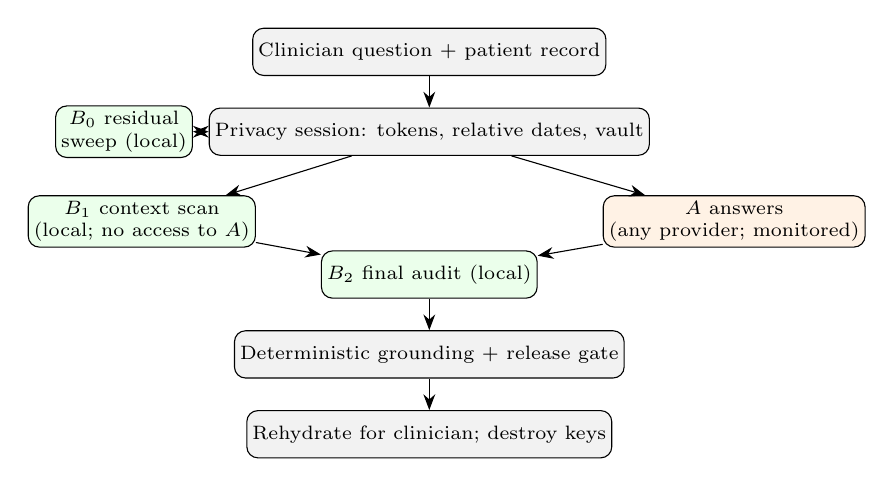
\begin{tikzpicture}[font=\scriptsize, node distance=4mm and 3mm,
  box/.style={draw, rounded corners, align=center, minimum height=6mm, inner sep=2pt},
  loc/.style={box, fill=green!8}, rem/.style={box, fill=orange!10}, det/.style={box, fill=gray!10},
  >={Stealth[length=2mm]}]
\node[det] (in) {Clinician question + patient record};
\node[det, below=of in] (p) {Privacy session: tokens, relative dates, vault};
\node[loc, below left=5mm and -6mm of p] (b1) {$B_1$ context scan\\(local; no access to $A$)};
\node[rem, below right=5mm and -6mm of p] (a) {$A$ answers\\(any provider; monitored)};
\node[loc, left=2mm of p] (b0) {$B_0$ residual\\sweep (local)};
\node[loc, below=12mm of p] (b2) {$B_2$ final audit (local)};
\node[det, below=of b2] (g) {Deterministic grounding + release gate};
\node[det, below=of g] (out) {Rehydrate for clinician; destroy keys};
\draw[->] (in) -- (p); \draw[->] (p) -- (b1); \draw[->] (p) -- (a);
\draw[<->, dashed] (b0) -- (p);
\draw[->] (b1) -- (b2); \draw[->] (a) -- (b2); \draw[->] (b2) -- (g); \draw[->] (g) -- (out);
\end{tikzpicture}}
\caption{Dual-lobe information flow. Green: must run locally. Orange: may run remotely, receives only de-identified data. Grey: deterministic, in-process.}
\label{fig:arch}
\end{figure}

\section{Formal Control Logic}
\subsection{Grounding}
Let $S=\{Q{:}\,q', A{:}\,a\}\cup\{F_1,\dots,F_n\}$ and let $K$ be the knowledge snippets retrieved for the request. A finding $h$ with kind $\kappa$, cited references $E$, knowledge references $E_K$ and quote $u$ is \emph{grounded} iff (i) $E\subseteq S$ and $E_K\subseteq K$; (ii) $E$ contains a record fact if $\kappa\in\{$unasked hazard, answer error$\}$, a fact or $Q$ if $\kappa=$ missing information, and $A$ if $\kappa=$ unsupported claim; and (iii) if $u\neq\varnothing$, $\mathrm{norm}(u)$ is a substring of $\mathrm{norm}(s)$ for some cited $s$. Fabricated references or quotes make $h$ ungrounded.

\subsection{Effective verdict and release gate}
GREEN is downgraded to YELLOW while any grounded finding or open evidence gap remains; RED is downgraded unless supported by a grounded answer error or grounded critical finding. The release gate (Table~\ref{tab:gate}) is evaluated in order.

\begin{table}[!t]
\caption{Release gate (first matching rule wins).}
\label{tab:gate}
\centering\footnotesize
\begin{tabular}{@{}p{0.3cm}p{4.2cm}p{2.9cm}@{}}
\toprule
\# & Condition & Release\\\midrule
1 & outbound call refused by privacy monitor & BLOCKED\\
2 & primary lobe produced no answer & UNVERIFIED$^\ast$\\
3 & no supervision (baseline arm) & UNSUPERVISED\\
4 & supervisor failed or unparsable & UNVERIFIED$^\ast$ (fail closed)\\
5 & grounded critical/major finding, or effective RED & HOLD\_FOR\_CLINICIAN$^\ast$\\
6 & effective YELLOW, or any other finding & RELEASE\_WITH\_ADVISORIES\\
7 & otherwise & RELEASE\\\bottomrule
\multicolumn{3}{@{}l}{$^\ast$Requires clinician acknowledgement.}
\end{tabular}
\end{table}

\subsection{Disagreement policy}
(1) Neither lobe overrides the other; the clinician arbitrates. (2) A disagreement interrupts only if grounded and rated critical or major; other objections are passive advisories, addressing alert fatigue \cite{ancker2017}. (3) On a hold, findings precede the answer, each with its source record entry, to counter automation bias \cite{goddard2012}. (4) Supervisory failure is visible, never a silent pass. (5) $B$ forms its view before seeing $A$'s answer. (6) Optionally, live challenges from $B$ reach $A$ during generation through a non-blocking channel.

\subsection{Evidence retrieval}
Patient evidence is the numbered fact list. Medical knowledge is retrieved deterministically from an institution-supplied corpus (formulary monographs, label excerpts, local guidelines) before $B$ is called, using the question and each fact as queries, and presented as numbered snippets; only retrieved identifiers may be cited. Retrieval thus does not depend on a local model's tool-use ability, and the evidence $B$ saw is fully known.

\subsection{Failure taxonomy}
$B$ reports four failure kinds of $A$---unasked hazard, missing information, answer error, unsupported claim---each rated critical (likely serious harm), major (should change the plan) or minor. Twelve system-level failure modes are controlled explicitly: supervisor miss, false alarm, fabricated evidence, malformed output, verdict inflation, automation bias, alert fatigue, identifier leakage, off-site supervisor, retention after use, correlated inter-lobe error, and primary failure (Table~\ref{tab:failures}).

\begin{table}[!t]
\caption{System failure modes and controls (abridged).}
\label{tab:failures}
\centering\footnotesize
\begin{tabular}{@{}p{2.6cm}p{5.1cm}@{}}
\toprule
Failure & Control\\\midrule
Supervisor false alarm & evidence-gated interruption; matched-twin measurement\\
Fabricated evidence & citation, quote and knowledge-ID verification\\
Malformed output & fail closed to UNVERIFIED\\
Automation bias & no edits to $A$; source entry shown; acknowledgement\\
Identifier leakage & de-identification, local sweep, two-layer egress monitor\\
Off-site supervisor & destination-based locality check; no failover\\
Retention after use & key destruction; no plaintext index; ephemeral memory\\
Correlated error & different conditioning; no shared context; distinct model\\\bottomrule
\end{tabular}
\end{table}

\section{Identity-Blind Inference}
A request-scoped session (i) registers structured identifiers under the HIPAA Safe Harbor categories \cite{hhs2012} and removes them from the view; (ii) propagates them, including capitalised name parts, into free text; (iii) detects pattern- and cue-based identifiers; (iv) converts dates to offsets from an index date and generalises ages over 89; (v) asks the local $B_0$ for residual identifiers, accepting only strings present verbatim; (vi) re-de-identifies every payload bound for a non-local destination at two layers---the runtime prompt and every framework message including tool results---refusing the call on failure; (vii) rehydrates tokens locally for display only; and (viii) destroys its keys when the request ends. The vault stores AES-256-GCM ciphertext \cite{nist38d} and a keyed HMAC-SHA256 index \cite{rfc2104}; no plaintext copy of an identifier is retained, tokens are random per request, and after key destruction nothing that outlived the request can be resolved or linked. $B$ is refused if its destination is not local, and has no failover to $A$'s provider.

\section{Analytical Properties}
Let $M$ denote ``$A$ misses the hazard'' and $D$ ``$B$ raises a grounded interrupting finding on it''. Then
\begin{equation}
P(\text{surfaced}) = P(\neg M) + P(M)\,P(D\mid M),
\end{equation}
so supervision adds exactly $P(M)P(D\mid M)$, which vanishes only if $B$'s misses coincide with $A$'s. Context conditioning, the pre-answer scan and a distinct local model target $P(D\mid M)$; the answer-verifier arm estimates their effect. Because a hold requires a grounded finding, every false hold is a misjudgement of a real, quoted record entry, never a fabrication. Wall-clock time is $T_{\text{sweep}}+\max(T_A,T_{\text{scan}})+T_{\text{audit}}$, the scan being concurrent with $A$.

\section{Evaluation Design}
\subsection{Benchmark and provenance}
The benchmark has 133 synthetic cases (Table~\ref{tab:bench}) in 17 clinical domains: drug--drug and drug--disease interactions; allergy and hypersensitivity; pregnancy, childbearing potential and lactation; renal and hepatic dosing; pharmacogenomics; QT prolongation; paediatric \cite{fda2017} and older-adult \cite{ags2023} prescribing; implanted devices; boxed warnings; red flags; unaddressed critical results; and missing dosing or baseline data. Forty of the 48 negative controls are \emph{matched twins}: the same question as a hazard case, with only the hazard fact removed. The other eight are independent controls, several with deliberate distractors. Each label records its label- or guideline-level basis; all identifiers are fictitious and planted in structured fields and narrative. A datasheet \cite{gebru2021} documents composition and provenance; every output row records the benchmark's SHA-256, code commit and model identifiers. Labels are validated by independent clinicians before the run: \pending{validators, specialties, agreement}. \pending{If the supervisory lobe is served through a hosted API for this synthetic study (no real patient data), state so; locality enforcement is verified separately by the integration tests.}

\begin{table}[!t]
\caption{Benchmark composition.}
\label{tab:bench}
\centering\footnotesize
\begin{tabular}{@{}lr@{}}
\toprule
Case type & $n$\\\midrule
Unasked hazard & 79\\
Missing information & 6\\
Negative control, independent (with distractors) & 8\\
Negative control, matched twin of a hazard case & 40\\\midrule
Total (planted identifiers: 626) & 133\\\bottomrule
\end{tabular}
\end{table}

\subsection{Arms, endpoints and statistics}
Three arms share the same models, de-identified view and retrieval: \emph{A only}; \emph{A + answer verifier} (same model, record and output schema as $B$, but answer-conditioned, without the pre-answer scan); and \emph{A + context-conditioned supervisor}. Each case is run \pending{$r\geq3$} times per arm. The primary endpoint is blinded adjudication by two clinicians of (i) whether the gold issue was surfaced, (ii) false alarm and (iii) harm if followed; disagreements go to a third clinician and agreement is reported as Cohen's $\kappa$. Secondary endpoints are automated screening sensitivity, false-hold rate, matched-pair discrimination (hold on the hazard version and not on its twin), repeat consistency, UNVERIFIED rate, planted-identifier leaks (a probe placed after the privacy monitor in every run), latency and model calls. Proportions carry Wilson intervals \cite{wilson1927}; arms are compared with the exact McNemar test \cite{mcnemar1947} on outcomes paired by case and repeat.

\section{Results}
\subsection{Control logic}
Exhaustive enumeration over supervision mode, privacy/primary/supervisor flags, seven verdict states, and every set of up to two findings drawn from 24 (kind\,$\times$\,severity\,$\times$\,grounded) types---50\,568 configurations---confirmed seven invariants: privacy dominates; fail closed; no hold without grounded evidence; every grounded critical/major finding holds; ungrounded findings never interrupt; a clean release implies no findings, no open gaps and GREEN; no finding is dropped.

\subsection{Privacy}
Table~\ref{tab:privacy} reports a deterministic audit of the exact text the answering model receives. Integration tests intercepting every payload at the provider boundary confirmed that no planted identifier reached the remote lobe, that the residual sweep and all supervisory calls reached only the local model, and that a configuration with a remote supervisor was refused before any payload left.

\begin{table}[!t]
\caption{Deterministic privacy audit (133 cases).}
\label{tab:privacy}
\centering\footnotesize
\begin{tabular}{@{}lr@{}}
\toprule
Identifiers planted & 626\\
Removed by deterministic layer & 624\\
Leaks attributable to deterministic layer & 0\\
Left for local residual sweep (uncued place name) & 2\\
Clinical values delivered unchanged & 385/385\\
Sessions with keys destroyed & 133/133\\\bottomrule
\end{tabular}
\end{table}

\subsection{Supervisory performance}
\pending{Table: per arm---surfaced (95\% CI), interrupted by $B$, false holds on negative controls (95\% CI), matched-pair discrimination, repeat consistency, UNVERIFIED, identifier leaks, median latency; McNemar $p$ for supervisor vs answer verifier and vs A only; Cohen's $\kappa$. Models: A = \dots, B = \dots, accessed \dots.}

\section{Discussion}
The central claim is narrow and testable: a supervisor conditioned on the whole record, formed before seeing the answer, surfaces omitted hazards that an answer-conditioned verifier with the same model and information does not, while discriminating hazard from matched no-hazard records. False alarms are treated as a first-class harm and automation bias as a design constraint: the supervisor never edits the answer and always points to the record entry behind an interruption. The dual-lobe split also carries the privacy argument: only a local model may read text before it is cleared to leave, making the supervisor the natural residual de-identifier---a role neither rules \cite{stubbs2015,neamatullah2008} nor a remote model can fill. \pending{interpretation of results, including unfavourable ones}.

\section{Limitations}
Cases are synthetic, short and author-written; labels require clinician validation. With 85 hazard cases the paired design detects moderate between-arm differences; repeats are not independent samples, and external validity requires real incident reports. Automated scoring is a screen; adjudication is primary. The privacy audit is in-sample and is not an estimate of de-identification recall, which should be measured on a standard corpus \cite{stubbs2015}; quasi-identifiers in narrative remain \cite{sweeney2000}; Python cannot guarantee erasure of transient string copies. Effects on clinician behaviour require a user study. The system is research software, not a medical device.

\section{Conclusion}
We turned the intuition that a clinical safety layer should look beyond the literal question into a specified, exhaustively verified and privacy-preserving architecture, with an evaluation that isolates context conditioning against a same-model verifier. Code, prompts, benchmark, datasheet and evaluation scripts are available at \url{https://github.com/anasalsawy/dual-lobe-clinical-safety}.

\begin{thebibliography}{99}
\bibitem{graber2005} M. L. Graber, N. Franklin, and R. Gordon, ``Diagnostic error in internal medicine,'' \emph{Arch. Intern. Med.}, vol. 165, no. 13, pp. 1493--1499, 2005.
\bibitem{singhal2023} K. Singhal \emph{et al.}, ``Large language models encode clinical knowledge,'' \emph{Nature}, vol. 620, pp. 172--180, 2023.
\bibitem{singhal2025} K. Singhal \emph{et al.}, ``Toward expert-level medical question answering with large language models,'' \emph{Nat. Med.}, vol. 31, pp. 943--950, 2025.
\bibitem{nori2023} H. Nori \emph{et al.}, ``Capabilities of GPT-4 on medical challenge problems,'' arXiv:2303.13375, 2023.
\bibitem{pal2023} A. Pal, L. K. Umapathi, and M. Sankarasubbu, ``Med-HALT: Medical domain hallucination test for large language models,'' in \emph{Proc. CoNLL}, 2023.
\bibitem{bai2022} Y. Bai \emph{et al.}, ``Constitutional AI: Harmlessness from AI feedback,'' arXiv:2212.08073, 2022.
\bibitem{madaan2023} A. Madaan \emph{et al.}, ``Self-Refine: Iterative refinement with self-feedback,'' in \emph{Proc. NeurIPS}, 2023.
\bibitem{shinn2023} N. Shinn \emph{et al.}, ``Reflexion: Language agents with verbal reinforcement learning,'' in \emph{Proc. NeurIPS}, 2023.
\bibitem{wang2023} X. Wang \emph{et al.}, ``Self-consistency improves chain of thought reasoning in language models,'' in \emph{Proc. ICLR}, 2023.
\bibitem{dhuliawala2024} S. Dhuliawala \emph{et al.}, ``Chain-of-verification reduces hallucination in large language models,'' in \emph{Findings ACL}, 2024.
\bibitem{cobbe2021} K. Cobbe \emph{et al.}, ``Training verifiers to solve math word problems,'' arXiv:2110.14168, 2021.
\bibitem{lightman2024} H. Lightman \emph{et al.}, ``Let's verify step by step,'' in \emph{Proc. ICLR}, 2024.
\bibitem{zheng2023} L. Zheng \emph{et al.}, ``Judging LLM-as-a-judge with MT-Bench and Chatbot Arena,'' in \emph{Proc. NeurIPS Datasets and Benchmarks}, 2023.
\bibitem{inan2023} H. Inan \emph{et al.}, ``Llama Guard: LLM-based input-output safeguard for human-AI conversations,'' arXiv:2312.06674, 2023.
\bibitem{rebedea2023} T. Rebedea \emph{et al.}, ``NeMo Guardrails: A toolkit for controllable and safe LLM applications with programmable rails,'' in \emph{Proc. EMNLP: System Demonstrations}, 2023.
\bibitem{du2024} Y. Du, S. Li, A. Torralba, J. B. Tenenbaum, and I. Mordatch, ``Improving factuality and reasoning in language models through multiagent debate,'' in \emph{Proc. ICML}, 2024.
\bibitem{irving2018} G. Irving, P. Christiano, and D. Amodei, ``AI safety via debate,'' arXiv:1805.00899, 2018.
\bibitem{bates2003} D. W. Bates \emph{et al.}, ``Ten commandments for effective clinical decision support,'' \emph{J. Am. Med. Inform. Assoc.}, vol. 10, no. 6, pp. 523--530, 2003.
\bibitem{sutton2020} R. T. Sutton \emph{et al.}, ``An overview of clinical decision support systems: Benefits, risks, and strategies for success,'' \emph{npj Digit. Med.}, vol. 3, art. 17, 2020.
\bibitem{vandersijs2006} H. van der Sijs, J. Aarts, A. Vulto, and M. Berg, ``Overriding of drug safety alerts in computerized physician order entry,'' \emph{J. Am. Med. Inform. Assoc.}, vol. 13, no. 2, pp. 138--147, 2006.
\bibitem{ancker2017} J. S. Ancker \emph{et al.}, ``Effects of workload, work complexity, and repeated alerts on alert fatigue in a clinical decision support system,'' \emph{BMC Med. Inform. Decis. Mak.}, vol. 17, art. 36, 2017.
\bibitem{carlini2021} N. Carlini \emph{et al.}, ``Extracting training data from large language models,'' in \emph{Proc. USENIX Security}, 2021.
\bibitem{tversky1974} A. Tversky and D. Kahneman, ``Judgment under uncertainty: Heuristics and biases,'' \emph{Science}, vol. 185, no. 4157, pp. 1124--1131, 1974.
\bibitem{vasey2022} B. Vasey \emph{et al.}, ``Reporting guideline for the early-stage clinical evaluation of decision support systems driven by artificial intelligence: DECIDE-AI,'' \emph{Nat. Med.}, vol. 28, pp. 924--933, 2022.
\bibitem{gallifant2025} J. Gallifant \emph{et al.}, ``The TRIPOD-LLM reporting guideline for studies using large language models,'' \emph{Nat. Med.}, vol. 31, pp. 60--69, 2025.
\bibitem{huang2024} J. Huang \emph{et al.}, ``Large language models cannot self-correct reasoning yet,'' in \emph{Proc. ICLR}, 2024.
\bibitem{greenblatt2024} R. Greenblatt, B. Shlegeris, K. Sachan, and F. Roger, ``AI control: Improving safety despite intentional subversion,'' in \emph{Proc. ICML}, 2024.
\bibitem{tang2024} X. Tang \emph{et al.}, ``MedAgents: Large language models as collaborators for zero-shot medical reasoning,'' in \emph{Findings ACL}, 2024.
\bibitem{kim2024} Y. Kim \emph{et al.}, ``MDAgents: An adaptive collaboration of LLMs for medical decision-making,'' in \emph{Proc. NeurIPS}, 2024.
\bibitem{lewis2020} P. Lewis \emph{et al.}, ``Retrieval-augmented generation for knowledge-intensive NLP tasks,'' in \emph{Proc. NeurIPS}, 2020.
\bibitem{zakka2024} C. Zakka \emph{et al.}, ``Almanac---Retrieval-augmented language models for clinical medicine,'' \emph{NEJM AI}, vol. 1, no. 2, 2024.
\bibitem{goddard2012} K. Goddard, A. Roudsari, and J. C. Wyatt, ``Automation bias: A systematic review of frequency, effect mediators, and mitigators,'' \emph{J. Am. Med. Inform. Assoc.}, vol. 19, no. 1, pp. 121--127, 2012.
\bibitem{parasuraman1997} R. Parasuraman and V. Riley, ``Humans and automation: Use, misuse, disuse, abuse,'' \emph{Hum. Factors}, vol. 39, no. 2, pp. 230--253, 1997.
\bibitem{sharma2024} M. Sharma \emph{et al.}, ``Towards understanding sycophancy in language models,'' in \emph{Proc. ICLR}, 2024.
\bibitem{hhs2012} U.S. Dept. of Health and Human Services, ``Guidance regarding methods for de-identification of protected health information in accordance with the HIPAA Privacy Rule,'' 2012; 45 CFR \S164.514(b)(2).
\bibitem{nist38d} M. Dworkin, ``Recommendation for block cipher modes of operation: Galois/Counter Mode (GCM) and GMAC,'' NIST SP 800-38D, 2007.
\bibitem{rfc2104} H. Krawczyk, M. Bellare, and R. Canetti, ``HMAC: Keyed-hashing for message authentication,'' RFC 2104, 1997.
\bibitem{fda2017} U.S. Food and Drug Administration, ``FDA restricts use of prescription codeine pain and cough medicines and tramadol pain medicines in children,'' Drug Safety Communication, Apr. 2017.
\bibitem{ags2023} 2023 American Geriatrics Society Beers Criteria Update Expert Panel, ``American Geriatrics Society 2023 updated AGS Beers Criteria for potentially inappropriate medication use in older adults,'' \emph{J. Am. Geriatr. Soc.}, vol. 71, no. 7, pp. 2052--2081, 2023.
\bibitem{gebru2021} T. Gebru \emph{et al.}, ``Datasheets for datasets,'' \emph{Commun. ACM}, vol. 64, no. 12, pp. 86--92, 2021.
\bibitem{wilson1927} E. B. Wilson, ``Probable inference, the law of succession, and statistical inference,'' \emph{J. Am. Stat. Assoc.}, vol. 22, pp. 209--212, 1927.
\bibitem{mcnemar1947} Q. McNemar, ``Note on the sampling error of the difference between correlated proportions or percentages,'' \emph{Psychometrika}, vol. 12, pp. 153--157, 1947.
\bibitem{stubbs2015} A. Stubbs, C. Kotfila, and \"{O}. Uzuner, ``Automated systems for the de-identification of longitudinal clinical narratives: Overview of 2014 i2b2/UTHealth shared task Track 1,'' \emph{J. Biomed. Inform.}, vol. 58, suppl., pp. S11--S19, 2015.
\bibitem{neamatullah2008} I. Neamatullah \emph{et al.}, ``Automated de-identification of free-text medical records,'' \emph{BMC Med. Inform. Decis. Mak.}, vol. 8, art. 32, 2008.
\bibitem{sweeney2000} L. Sweeney, ``Simple demographics often identify people uniquely,'' Carnegie Mellon Univ., Data Privacy Working Paper 3, 2000.
\end{thebibliography}

\end{document}
